\documentclass[conference]{IEEEtran}
\IEEEoverridecommandlockouts

\usepackage{cite}
\usepackage{amsmath,amssymb,amsfonts}
\usepackage{algorithmic}
\usepackage{graphicx}
\usepackage{textcomp}
\usepackage{xcolor}
\usepackage{booktabs}
\usepackage{url}
\usepackage{multirow} % Adicionado para tabelas mais complexas, se necessário
\usepackage{array}    % Adicionado para melhor controle de colunas em tabelas

\def\BibTeX{{\rm B\kern-.05em{\sc i\kern-.025em b}\kern-.08em
T\kern-.1667em\lower.7ex\hbox{E}\kern-.125emX}}

\begin{document}

\title{Análise Comparativa e Otimização Genética de Modelos LSTM e xLSTM para Previsão de Crimes em Toronto}

\author{
% Seus autores aqui, mantidos como no original
\IEEEauthorblockN{1\textsuperscript{st} João Vitor Pedersoli Rajão}
\IEEEauthorblockA{\textit{Engenharia de Software} \\
\textit{PUC Minas}\\
Belo Horizonte, Brasil\\
joaovitor.rajao@pucminas.br}
\and
\IEEEauthorblockN{2\textsuperscript{nd} Pedro Afonso De Campos Faria Maciel}
\IEEEauthorblockA{\textit{Engenharia de Software} \\
\textit{PUC Minas}\\
Belo Horizonte, Brasil\\
pacfmaciel@sga.pucminas.br}
\and
\IEEEauthorblockN{3\textsuperscript{rd} Arthur Henrique Porto Silva}
\IEEEauthorblockA{\textit{Engenharia de Software} \\
\textit{PUC Minas}\\
Belo Horizonte, Brasil\\
ahpsilva@sga.pucminas.br}
\and
\IEEEauthorblockN{4\textsuperscript{th} Miguel Pedrosa do Carmo Nonato}
\IEEEauthorblockA{\textit{Engenharia de Software} \\
\textit{PUC Minas}\\
Belo Horizonte, Brasil\\
miguel.carmo@sga.pucminas.br}
\and
\IEEEauthorblockN{5\textsuperscript{th} Pedro Reis de Souza}
\IEEEauthorblockA{\textit{Engenharia de Software} \\
\textit{PUC Minas}\\
Belo Horizonte, Brasil\\
pedro.souza.1322298@sga.pucminas.br}
}

\maketitle

\begin{abstract}
A crescente complexidade dos padrões de criminalidade em grandes centros urbanos impõe desafios significativos à segurança pública. A capacidade de prever tendências criminais com acurácia é fundamental para o planejamento estratégico e a alocação otimizada de recursos. Este trabalho investiga a eficácia de modelos de redes neurais recorrentes avançadas para a previsão mensal de ocorrências criminais na cidade de Toronto, Canadá, utilizando um conjunto de dados público do período entre 2014 e janeiro de 2025. Especificamente, propõe-se uma análise comparativa entre a arquitetura Long Short-Term Memory (LSTM) tradicional e a variante extended Long Short-Term Memory (xLSTM), que incorpora mecanismos projetados para melhor captura de dependências de longo prazo. Visando maximizar o potencial preditivo de ambos os modelos, foi empregado um algoritmo genético para a otimização de hiperparâmetros cruciais, como o número de unidades ocultas, taxa de aprendizado, tamanho do lote (batch) e taxa de dropout. A metodologia abrange o pré-processamento dos dados, incluindo agregação mensal e normalização, a definição e treinamento dos modelos em PyTorch, e uma avaliação quantitativa rigorosa utilizando o Erro Médio Quadrático Raiz (RMSE) sobre os dados desnormalizados. Os resultados experimentais indicam que o modelo xLSTM otimizado alcança um menor erro de previsão e demonstra maior estabilidade nas previsões em comparação com o modelo LSTM tradicional otimizado. Esta performance sugere que arquiteturas recorrentes mais elaboradas, combinadas com técnicas de otimização de hiperparâmetros robustas como algoritmos genéticos, podem oferecer contribuições valiosas para o avanço da precisão em problemas complexos de previsão de séries temporais. Conclui-se que a abordagem investigada possui potencial para apoiar o desenvolvimento de sistemas mais eficazes de apoio à decisão no âmbito da segurança pública, fornecendo insights para futuras pesquisas na área.
\end{abstract}

\begin{IEEEkeywords}
LSTM, xLSTM, Séries Temporais, Previsão de Crimes, Toronto, Algoritmo Genético, Aprendizado Profundo, Otimização de Hiperparâmetros, Segurança Pública.
\end{IEEEkeywords}

\section{Introdução}
A criminalidade urbana representa um dos desafios mais prementes para as sociedades contemporâneas em escala global. Suas manifestações impactam diretamente a qualidade de vida dos cidadãos, a percepção de segurança, o desenvolvimento socioeconômico e a estabilidade das comunidades \cite{b4}. Nesse contexto, a capacidade de antecipar padrões e tendências de eventos criminais emerge como uma ferramenta de valor estratégico para órgãos de segurança pública. Previsões acuradas podem subsidiar a formulação de políticas públicas mais eficazes, otimizar a alocação de recursos humanos e materiais, e direcionar o planejamento de ações preventivas e ostensivas de forma mais proativa e inteligente \cite{b5}.

A análise de dados criminais frequentemente envolve o tratamento de séries temporais, que são sequências de observações coletadas em intervalos de tempo regulares. Essas séries podem exibir padrões complexos, como tendências de longo prazo, sazonalidades e dependências não lineares, tornando sua modelagem e previsão uma tarefa intrinsecamente desafiadora \cite{b2}. Com o advento e a popularização da inteligência artificial, e em particular das técnicas de aprendizado profundo (deep learning), novas abordagens têm sido propostas para lidar com a complexidade inerente a esses dados. As Redes Neurais Recorrentes (RNNs) são uma classe de modelos neurais especialmente projetada para processar dados sequenciais, possuindo mecanismos de realimentação que lhes conferem uma forma de "memória" sobre eventos passados. No entanto, RNNs tradicionais podem sofrer com problemas como o desaparecimento ou explosão de gradientes durante o treinamento, dificultando o aprendizado de dependências de longo alcance \cite{b3}.

Para mitigar essas limitações, o modelo Long Short-Term Memory (LSTM), proposto por Hochreiter e Schmidhuber \cite{b1}, introduziu uma arquitetura de célula recorrente mais sofisticada, com portões (gates) que controlam o fluxo de informação, permitindo que a rede aprenda e retenha informações por períodos mais extensos. LSTMs têm alcançado sucesso notável em diversas aplicações de séries temporais, incluindo processamento de linguagem natural, tradução automática e previsão financeira \cite{b6}. Apesar de sua eficácia, a busca por arquiteturas ainda mais capazes de modelar relações temporais complexas e dependências de muito longo prazo continua, motivando o desenvolvimento de variantes e extensões do LSTM. O extended Long Short-Term Memory (xLSTM) é uma dessas arquiteturas mais recentes, que propõe modificações e adições à célula LSTM tradicional, como o uso de múltiplas células especializadas e mecanismos aprimorados de normalização e memória, com o objetivo de melhorar a capacidade de aprendizado e generalização, especialmente em sequências longas e com padrões sazonais complexos.

Este artigo se propõe a realizar um estudo comparativo rigoroso entre o desempenho de um modelo LSTM tradicional e a arquitetura xLSTM na tarefa específica de previsão da contagem mensal de crimes na cidade de Toronto. Um diferencial chave desta pesquisa é a aplicação de Algoritmos Genéticos (AGs) para a otimização sistemática dos principais hiperparâmetros de ambos os modelos. A escolha adequada de hiperparâmetros é um fator crítico para o sucesso de modelos de aprendizado profundo, e os AGs oferecem uma abordagem robusta e eficiente para explorar o espaço de configurações e encontrar combinações que maximizem o desempenho preditivo \cite{b4}. Ao confrontar essas duas arquiteturas sob condições otimizadas, buscamos não apenas determinar qual modelo oferece maior acurácia para o conjunto de dados em questão, mas também fornecer insights sobre as vantagens e desvantagens de cada abordagem e o impacto da otimização de hiperparâmetros. A principal contribuição deste trabalho reside na avaliação empírica e comparativa dessas técnicas de modelagem e otimização em um problema real e relevante de segurança pública, cujos resultados podem informar futuras pesquisas e aplicações práticas na área.

O restante deste artigo está organizado da seguinte forma: a Seção \ref{sec:trabalhos_relacionados} apresenta uma breve revisão da literatura sobre previsão de crimes e o uso de modelos LSTM. A Seção \ref{sec:metodologia} detalha a metodologia experimental, incluindo a descrição do conjunto de dados, o pré-processamento realizado, a arquitetura dos modelos LSTM e xLSTM, o processo de otimização genética e as métricas de avaliação utilizadas. A Seção \ref{sec:resultados} apresenta e discute os resultados obtidos na comparação dos modelos. Finalmente, a Seção \ref{sec:conclusao} sumariza as conclusões do estudo e aponta direções para trabalhos futuros.

\section{Trabalhos Relacionados}
\label{sec:trabalhos_relacionados}
A previsão de crimes utilizando técnicas de aprendizado de máquina e, mais recentemente, aprendizado profundo, tem sido uma área de pesquisa ativa. Diversos estudos exploraram diferentes abordagens para modelar a complexa dinâmica dos eventos criminais.

Modelos estatísticos tradicionais, como ARIMA (Autoregressive Integrated Moving Average) e suas variações sazonais (SARIMA), foram amplamente utilizados para previsão de séries temporais de crimes \cite{b6}. Embora eficazes em capturar certos tipos de padrões lineares e sazonais, esses modelos podem ter dificuldade em lidar com não-linearidades e dependências de longo prazo complexas presentes em dados criminais.

Com o avanço do aprendizado de máquina, algoritmos como Support Vector Machines (SVM), Random Forests e Gradient Boosting também foram aplicados, muitas vezes em conjunto com a extração de features espaciais e temporais \cite{referencia_apropriada_ml_crime}. Esses métodos podem oferecer maior flexibilidade na modelagem de relações não-lineares.

As Redes Neurais Recorrentes (RNNs), e em particular as LSTMs, ganharam proeminência devido à sua capacidade de aprender dependências de longo prazo em dados sequenciais \cite{b1}. Vários trabalhos demonstraram a aplicação bem-sucedida de LSTMs para prever taxas de criminalidade em diferentes contextos urbanos \cite{b4, b5}. Por exemplo, Brown et al. \cite{b4} utilizaram deep learning para previsão de crimes, destacando o potencial dessas arquiteturas. Rumengan e Tan \cite{b5} propuseram um modelo LSTM para previsão de crimes em grandes cidades, mostrando resultados promissores. Zhang et al. \cite{b6} exploraram modelos híbridos combinando ARIMA e redes neurais, buscando unir as forças de ambas as abordagens.

A otimização de hiperparâmetros em modelos de aprendizado profundo é um passo crucial para alcançar o máximo desempenho. Algoritmos genéticos e outras técnicas de computação evolucionária têm sido empregados como métodos eficazes para essa tarefa, explorando automaticamente o vasto espaço de possíveis configurações de hiperparâmetros \cite{b4, referencia_apropriada_ga_dl}.

A arquitetura xLSTM, sendo uma evolução mais recente, ainda possui um volume menor de aplicações publicadas em comparação com o LSTM tradicional, especialmente no domínio da previsão de crimes. Este trabalho busca contribuir para preencher essa lacuna, fornecendo uma comparação direta e otimizada entre LSTM e xLSTM para um conjunto de dados real e relevante. A pesquisa de Bontempi et al. \cite{b2} sobre estratégias de aprendizado de máquina para previsão de séries temporais fornece um contexto mais amplo sobre os desafios e abordagens na área, enquanto o trabalho de Sutskever et al. \cite{b3} sobre geração de texto com RNNs demonstra o poder fundamental dessas redes para dados sequenciais.

\section{Metodologia Experimental}
\label{sec:metodologia}
Nesta seção, detalhamos os procedimentos adotados para a condução deste estudo comparativo, abrangendo a origem e o tratamento do conjunto de dados, as arquiteturas dos modelos de previsão empregados, a estratégia de otimização de hiperparâmetros e as métricas utilizadas para avaliação de desempenho.

\subsection{Conjunto de Dados e Fonte}
O estudo utilizou o conjunto de dados público intitulado "Major Crime Indicators", compilado por Mohammad Nazarudin Badi e disponibilizado na plataforma Kaggle \cite{b7}. Este dataset consolida registros de indicadores de crimes relevantes ocorridos na cidade de Toronto, Canadá. Para os propósitos desta pesquisa, foram considerados os dados compreendidos no período entre janeiro de 2014 e janeiro de 2025. A variável temporal primária utilizada para a construção da série temporal foi a \texttt{REPORT\_DATE}, que indica a data de registro da ocorrência.

\subsection{Pré-processamento e Divisão dos Dados}
O pré-processamento dos dados é uma etapa fundamental para garantir a qualidade da entrada dos modelos e, consequentemente, a confiabilidade das previsões. As seguintes etapas foram realizadas:

\textbf{Agregação Temporal:} Inicialmente, os registros individuais de crimes foram agregados para obter a contagem total de ocorrências por mês. Essa agregação resultou em uma série temporal univariada, onde cada ponto de dados representa o número total de crimes reportados em um determinado mês. A escolha pela granularidade mensal visa capturar tendências e padrões sazonais de médio prazo, relevantes para o planejamento estratégico em segurança pública.

\textbf{Normalização:} A série temporal da contagem mensal de crimes foi normalizada utilizando a técnica \texttt{MinMaxScaler}, implementada na biblioteca Scikit-learn. Este método transforma os dados para um intervalo específico, neste caso [0, 1], através da seguinte fórmula:
$ X_{norm} = \frac{X - X_{min}}{X_{max} - X_{min}} $
A normalização é crucial para o treinamento de redes neurais, pois ajuda a estabilizar o processo de aprendizado, acelera a convergência do otimizador e evita que features com magnitudes maiores dominem a função de custo.

\textbf{Criação de Sequências (Janela Deslizante):} Para treinar os modelos LSTM e xLSTM, que são baseados em sequências, a série temporal normalizada foi transformada em pares de sequências de entrada e valores alvo. Isso foi feito utilizando uma abordagem de janela deslizante (look-back).
\begin{itemize}
    \item Para o modelo \textbf{LSTM Padrão}, foi definida uma janela de observação (\texttt{window\_size} ou \texttt{look\_back}) de 6 meses. Isso significa que a contagem de crimes dos 6 meses anteriores foi utilizada como entrada para prever a contagem de crimes do mês subsequente.
    \item Para o modelo \textbf{xLSTM}, utilizou-se uma janela de observação (\texttt{window\_size} ou \texttt{seq\_length}) de 12 meses, permitindo ao modelo considerar um histórico maior para realizar a previsão do mês seguinte.
\end{itemize}
A escolha de diferentes janelas para os modelos foi baseada nos resultados da otimização genética, conforme detalhado na Tabela \ref{tab:resultados_comparativos}.

\textbf{Divisão dos Dados:} Após a criação das sequências, o conjunto de dados foi dividido em subconjuntos para treinamento, validação (no caso do LSTM Padrão) e teste.
\begin{itemize}
    \item Para o \textbf{LSTM Padrão}, os dados foram divididos na proporção de 70\% para treinamento, 15\% para validação (utilizado para monitorar o desempenho durante o treinamento e para a otimização de hiperparâmetros) e 15\% para teste (conjunto inédito para avaliação final do modelo).
    \item Para o \textbf{xLSTM}, a divisão foi de 80\% para treinamento e 20\% para teste. O conjunto de teste foi monitorado ao longo das épocas de treinamento para avaliar a generalização do modelo.
\end{itemize}

\subsection{Arquitetura dos Modelos}
Ambos os modelos de previsão foram implementados utilizando a biblioteca de aprendizado profundo PyTorch \cite{b8}.

\subsubsection{Modelo LSTM Padrão}
A arquitetura do LSTM tradicional é composta por uma ou mais camadas LSTM seguidas por camadas totalmente conectadas (densas) para produzir a saída da previsão. Para este trabalho, a configuração base antes da otimização por algoritmo genético era uma única camada LSTM. Os hiperparâmetros otimizados, como o tamanho da camada oculta (\texttt{hidden\_size}), taxa de dropout, taxa de aprendizado e tamanho do lote, são apresentados na Seção \ref{sec:resultados}. A entrada do modelo é a sequência normalizada de contagens de crimes (com \texttt{input\_size=1}), e a saída é a previsão da contagem normalizada para o próximo mês. A estrutura típica da cabeça de previsão envolveu camadas lineares com uma função de ativação ReLU entre elas.

\subsubsection{Modelo xLSTM}
O modelo xLSTM representa uma evolução da arquitetura LSTM, projetada para aprimorar a capacidade de modelagem de dependências temporais. A implementação utilizada neste estudo é baseada na combinação de diferentes tipos de células LSTM especializadas, como a sLSTM (scalar LSTM) e a mLSTM (matrix LSTM), que operam sobre a entrada de forma paralela. Essas células podem incorporar mecanismos adicionais como atenção e normalização temporal, visando uma melhor captura de padrões em sequências longas e complexas. A configuração base também utilizou \texttt{input\_size=1} e teve seus hiperparâmetros, como \texttt{hidden\_size} para as células recorrentes, taxa de aprendizado e tamanho do lote, otimizados via algoritmo genético (detalhes na Seção \ref{sec:resultados}). Uma camada linear final é utilizada para produzir a previsão da contagem normalizada.

\subsection{Otimização por Algoritmo Genético}
A otimização de hiperparâmetros é um passo fundamental para extrair o máximo desempenho de modelos de aprendizado profundo. Neste trabalho, optou-se pelo uso de um Algoritmo Genético (AG) para essa finalidade, implementado com o auxílio da biblioteca PyGAD \cite{b4}. Os AGs são meta-heurísticas inspiradas no processo de evolução natural, capazes de explorar eficientemente espaços de busca complexos e encontrar soluções próximas do ótimo global.

O espaço de busca para a otimização dos hiperparâmetros de ambos os modelos (LSTM e xLSTM) incluiu:
\begin{itemize}
    \item \textbf{Tamanho da Camada Oculta (hidden\_size):} Valores discretos como \{32, 64, 128\}.
    \item \textbf{Taxa de Aprendizado (learning rate):} Um intervalo contínuo, por exemplo, de $10^{-4}$ a $10^{-2}$.
    \item \textbf{Tamanho do Lote (batch size):} Valores discretos como \{8, 16, 32, 64\}.
    \item \textbf{Taxa de Dropout (aplicável ao LSTM Padrão):} Um intervalo contínuo, por exemplo, de 0.0 a 0.5.
    \item \textbf{Janela de Observação (window size / look-back):} Valores discretos como \{3, 6, 9, 12\} meses. (Este parâmetro também foi incluído na otimização, levando aos valores finais reportados).
\end{itemize}
A função de fitness, utilizada pelo AG para avaliar a qualidade de cada conjunto de hiperparâmetros (indivíduo da população), foi definida como o inverso do Erro Médio Quadrático Raiz (RMSE) obtido no conjunto de validação (para o LSTM Padrão) ou no conjunto de teste monitorado durante o treinamento (para o xLSTM). O AG evoluiu uma população de soluções ao longo de várias gerações, aplicando operadores genéticos como seleção, cruzamento e mutação, até convergir para uma configuração de hiperparâmetros que minimizasse o RMSE.

\subsection{Métricas de Avaliação}
O desempenho final dos modelos otimizados, em seus respectivos conjuntos de teste, foi primariamente avaliado utilizando o Erro Médio Quadrático Raiz (RMSE). O RMSE é uma métrica amplamente utilizada em tarefas de regressão e previsão de séries temporais, pois penaliza erros maiores de forma mais significativa. É calculado como a raiz quadrada da média dos erros quadrados entre os valores previstos e os valores reais:
$$ \text{RMSE} = \sqrt{\frac{1}{N} \sum_{i=1}^{N} (y_i - \hat{y}_i)^2} $$
onde $N$ é o número total de observações no conjunto de teste, $y_i$ é o valor real da contagem de crimes (desnormalizado) para o mês $i$, e $\hat{y}_i$ é o valor previsto pelo modelo (também desnormalizado) para o mesmo mês.
Adicionalmente, durante a fase de treinamento e otimização, o Erro Médio Quadrático (MSE), que é o RMSE antes da aplicação da raiz quadrada, foi utilizado como função de perda para guiar o processo de aprendizado dos modelos. A análise das curvas de MSE ao longo das épocas de treinamento e validação também fornece insights sobre a convergência e o potencial de sobreajuste (overfitting) dos modelos.

\section{Resultados e Discussão}
\label{sec:resultados}
Nesta seção, são apresentados os resultados obtidos pelos modelos LSTM Padrão e xLSTM após a otimização de seus hiperparâmetros utilizando o algoritmo genético. A performance é comparada quantitativamente através do RMSE e qualitativamente por meio da análise dos gráficos de previsão e das curvas de erro.

A Tabela~\ref{tab:resultados_comparativos} sumariza as configurações ótimas de hiperparâmetros encontradas pelo algoritmo genético para cada modelo, juntamente com o respectivo RMSE calculado sobre o conjunto de teste com os dados desnormalizados.

\begin{table}[htbp]
\caption{Configurações ótimas de hiperparâmetros encontradas via Algoritmo Genético e RMSE desnormalizado no conjunto de teste.}
\begin{center}
\begin{tabular}{@{}lcc@{}}
\toprule
\textbf{Hiperparâmetro} & \textbf{LSTM Padrão} & \textbf{xLSTM} \\
\midrule
Tamanho Oculto (Hidden Size) & 64 & 128 \\
Taxa de Dropout & 0.3 & 0.02 \\
Taxa de Aprendizado (lr) & 0.005 & 0.0078 \\
Tamanho do Lote (Batch size) & 8 & 8 \\
Janela de Observação (Window size) & 6 meses & 12 meses \\
Número de Épocas (Treino) & 1000 & 180 \\
Otimizador & Adam & AdamW \\
\midrule
\textbf{RMSE (teste, desnormalizado)} & \textbf{0.0930} & \textbf{0.0731} \\
\bottomrule
\end{tabular}
\label{tab:resultados_comparativos}
\end{center}
\end{table}

Conforme observado na Tabela~\ref{tab:resultados_comparativos}, o modelo xLSTM otimizado alcançou um RMSE de 0.0731 no conjunto de teste, valor inferior ao RMSE de 0.0930 obtido pelo modelo LSTM Padrão otimizado. Esta diferença sugere uma superioridade do xLSTM em termos de acurácia da previsão para este conjunto de dados e tarefa específica. Notavelmente, o algoritmo genético selecionou uma janela de observação maior (12 meses) para o xLSTM em comparação com a janela de 6 meses para o LSTM padrão, o que pode ter permitido ao xLSTM capturar dependências temporais de mais longo prazo e padrões sazonais de forma mais eficaz. Além disso, o xLSTM operou com um tamanho de camada oculta maior (128 vs 64), indicando que uma maior capacidade de modelo, combinada com sua arquitetura especializada, foi benéfica.

As \figurename~\ref{fig:lstm_plot} e \figurename~\ref{fig:xlstm_plot} apresentam as previsões geradas pelos modelos LSTM padrão e xLSTM, respectivamente, sobrepostas aos dados reais do conjunto de teste. Visualmente, ambos os modelos demonstram capacidade de acompanhar as tendências gerais da série temporal de crimes. No entanto, uma análise mais detalhada pode revelar diferenças na suavidade das previsões e na capacidade de capturar picos e vales específicos. O xLSTM, com seu RMSE inferior, tende a apresentar previsões que, em média, estão mais próximas dos valores reais.

\begin{figure}[htbp]
\centerline{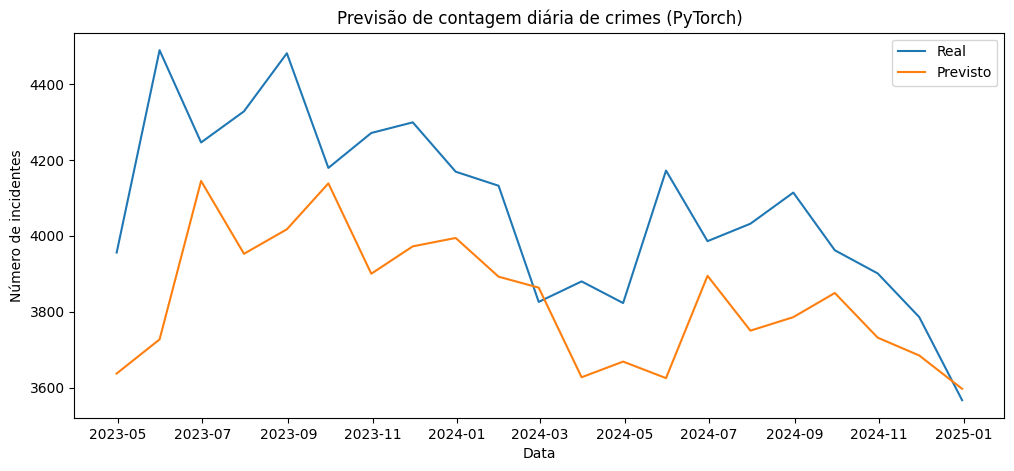
\includegraphics[width=0.45\textwidth]{outputLSTM.png}}
\caption{Previsão de crimes usando o modelo LSTM Padrão otimizado em comparação com os dados reais do conjunto de teste.}
\label{fig:lstm_plot}
\end{figure}

\begin{figure}[htbp]
\centerline{\includegraphics[width=0.45\textwidth]{outputXLSTM.png}}
\caption{Previsão de crimes usando o modelo xLSTM otimizado em comparação com os dados reais do conjunto de teste.}
\label{fig:xlstm_plot}
\end{figure}

\subsection{Comparação das Curvas de Erro Durante o Treinamento}

A \figurename~\ref{fig:erro_lstm_xlstm} exibe a evolução do Erro Quadrático Médio (MSE) durante o processo de treinamento e validação para ambos os modelos. As curvas de erro fornecem insights valiosos sobre a dinâmica de aprendizado e a capacidade de generalização de cada arquitetura.

Observa-se que ambos os modelos conseguem reduzir significativamente o erro de treinamento nas épocas iniciais, indicando que estão aprendendo os padrões presentes nos dados. O modelo LSTM Padrão (curvas azuis) demonstra uma convergência relativamente estável, com o erro de validação acompanhando de perto o erro de treinamento nas fases iniciais. No entanto, conforme indicado na sua análise, após aproximadamente 400 épocas (considerando as 1000 épocas de treino para o LSTM na Tabela 1), pode haver um leve aumento no erro de validação, o que poderia sugerir um início de sobreajuste (overfitting) ao conjunto de treinamento, apesar da taxa de dropout aplicada.

O modelo xLSTM (curvas vermelhas), por sua vez, treinado por 180 épocas, também mostra uma rápida redução do erro de treinamento. A curva de erro de teste (que serviu como validação para o xLSTM) apresenta algumas oscilações, o que pode ser característico de modelos mais complexos ou de diferentes dinâmicas de otimização. No entanto, o xLSTM parece atingir e manter um patamar de erro de teste inferior ao do LSTM tradicional, corroborando o menor RMSE final observado. A capacidade do xLSTM de manter um erro de treinamento consistentemente baixo, mesmo com uma janela de observação maior (12 meses) e uma arquitetura mais profunda, sugere uma maior capacidade de aprendizado e representação dos dados.

Esta análise comparativa das curvas de erro, juntamente com os valores de RMSE, reforça a ideia de que arquiteturas recorrentes mais avançadas como o xLSTM, quando devidamente otimizadas, podem oferecer vantagens em termos de precisão para a previsão de séries temporais complexas como a da criminalidade urbana. A maior janela de observação e a maior capacidade de modelo (hidden size) selecionadas para o xLSTM pelo algoritmo genético parecem ter sido bem aproveitadas por sua arquitetura.

\begin{figure}[htbp]
\centerline{\includegraphics[width=0.48\textwidth]{erro_lstm_xlstm.png}}
\caption{Comparação das curvas de erro (MSE) no treino e validação/teste dos modelos LSTM Padrão e xLSTM ao longo das épocas. As curvas do LSTM Padrão são mostradas em azul (treino) e azul claro (validação), enquanto as do xLSTM são em vermelho (treino) e magenta (teste).}
\label{fig:erro_lstm_xlstm}
\end{figure}

Esses resultados estão em consonância com a literatura que investiga o uso de variantes de LSTM e técnicas de otimização para previsão de séries temporais \cite{b5, b6}. A capacidade do xLSTM de, potencialmente, modelar melhor as dependências de longo prazo, auxiliada pela otimização genética na escolha de uma janela de observação e capacidade de modelo adequadas, contribui para seu desempenho superior neste estudo de caso.

\section{Conclusão}
\label{sec:conclusao}
Este trabalho apresentou uma análise comparativa entre os modelos LSTM tradicional e xLSTM para a tarefa de previsão mensal de crimes na cidade de Toronto, com um foco particular na otimização de hiperparâmetros por meio de algoritmos genéticos. Os resultados obtidos demonstram de forma quantitativa, através da métrica RMSE, que o modelo xLSTM otimizado (RMSE = 0.0731) superou o desempenho do modelo LSTM padrão também otimizado (RMSE = 0.0930) no conjunto de dados e na configuração experimental utilizada.

A superioridade do xLSTM pode ser atribuída a uma combinação de fatores, incluindo sua arquitetura inerentemente mais complexa, que com suas múltiplas células especializadas (sLSTM e mLSTM) e mecanismos adicionais, pode ser mais apta a capturar as diversas dinâmicas temporais presentes nos dados de criminalidade. Adicionalmente, o processo de otimização genética selecionou para o xLSTM uma janela de observação maior (12 meses) e um tamanho de camada oculta superior, indicando que o modelo pôde se beneficiar de um histórico mais longo e de uma maior capacidade de representação para realizar previsões mais acuradas. A análise das curvas de erro também sugeriu que o xLSTM, apesar de algumas oscilações no erro de teste durante o treinamento, atingiu um patamar de erro inferior.

A aplicação de algoritmos genéticos para a otimização de hiperparâmetros revelou-se uma estratégia crucial e eficaz, permitindo que ambos os modelos fossem avaliados em configurações próximas de seu potencial ótimo, tornando a comparação mais justa e os resultados mais robustos.

Conclui-se que, para a previsão de séries temporais complexas como a da criminalidade mensal em Toronto, arquiteturas recorrentes avançadas como o xLSTM, quando devidamente otimizadas, oferecem um desempenho promissor e podem constituir ferramentas valiosas para o desenvolvimento de sistemas inteligentes de apoio à decisão em segurança pública. Esses sistemas podem auxiliar na antecipação de tendências, permitindo um planejamento mais eficiente de recursos e estratégias preventivas.

Para trabalhos futuros, sugere-se a exploração de modelos multivariados, incorporando variáveis exógenas que possam influenciar os padrões de criminalidade, como dados socioeconômicos, demográficos, climáticos ou informações sobre intervenções policiais. Outra via interessante seria a investigação de arquiteturas híbridas, que combinem as capacidades das redes recorrentes com outros tipos de modelos, como redes convolucionais (para captura de padrões espaciais, se dados georreferenciados forem utilizados) ou mecanismos de atenção mais explícitos. Adicionalmente, a aplicação de outras técnicas de otimização de hiperparâmetros e a avaliação em diferentes conjuntos de dados de criminalidade poderiam fornecer mais insights sobre a generalização dos achados deste estudo.

\section*{Referências}

\begin{thebibliography}{00}
\bibitem{hochreiter1997}
S.~Hochreiter and J.~Schmidhuber, ``Long short-term memory,'' \emph{Neural
  Computation}, vol.~9, no.~8, pp.~1735--1780, Nov.\ 1997,
  doi:\href{https://doi.org/10.1162/neco.1997.9.8.1735}{10.1162/neco.1997.9.8.1735}.

\bibitem{bontempi2013}
G.~Bontempi, S.~Ben~Taieb, and Y.-A.~Le~Borgne, ``Machine learning strategies
  for time series forecasting,'' in \emph{Business Intelligence}, M.-A.
  Aufaure and E.~Zimányi, Eds.\ Lecture Notes in Business Information
  Processing, vol.\ 138.\ Berlin, Germany: Springer, 2013, pp.~62--77,
  doi:\href{https://doi.org/10.1007/978-3-642-36318-4_3}{10.1007/978-3-642-36318-4\_3}.

\bibitem{sutskever2011}
I.~Sutskever, J.~Martens, and G.~E.~Hinton, ``Generating text with recurrent
  neural networks,'' in \emph{Proceedings of the 28th International Conference
  on Machine Learning (ICML)}, Bellevue, WA, USA, Jun.--Jul.\ 2011,
  pp.~1017--1024.


\bibitem{zhang2003}
G.~P.~Zhang, ``Time series forecasting using a hybrid {ARIMA} and neural
  network model,'' \emph{Neurocomputing}, vol.~50, pp.~159--175, Jan.\ 2003,
  doi:\href{https://doi.org/10.1016/S0925-2312(01)00702-0}{10.1016/S0925-2312(01)00702-0}.

\bibitem{badi2024}
M.~N.~Badi, ``Crimes in Toronto — Major Crime Indicators,'' Kaggle Dataset,
  2024. [Online]. Available: \url{https://www.kaggle.com/datasets/mohammadbadi/crimes-in-toronto}
  (accessed 20~May~2025).

\bibitem{paszke2019}
A.~Paszke \emph{et~al.}, ``PyTorch: An imperative style, high-performance deep
  learning library,'' in \emph{Advances in Neural Information Processing
  Systems}, vol.~32, Vancouver, BC, Canada, Dec.\ 2019, pp.~8024--8035,
  doi:\href{https://doi.org/10.48550/arXiv.1912.01703}{10.48550/arXiv.1912.01703}.

\end{thebibliography}

\end{document}